\newpage
\section{Moderne Kryptographie}
Dieses Kapitel wurde mit Hilfe des Buches \textit{Moderne Verfahren der Kryptographie} erarbeitet.\\[2ex]
Die moderne Kryptographie unterscheidet sich von der klassischen Kryptographie in der Technik. Was früher von Hand errechnet wurde, wird in der modernen Kryptographie elektronisch erledigt. Mit dieser technischen Hilfe ist es möglich, komplexe Berechnungen in vernünftiger Zeit durchzuführen. Die grossen Chiffriermaschinen werden durch den Computer abgelöst.\\
Die immer besseren, beziehungsweise schnelleren Computer machen die klassische Kryptographie sehr unsicher, da der Schlüssel durch Brute-Force-Angriffe\footnote{Brute-Force nennt man dass Vorgehen, ein Passwort durch Ausprobieren aller möglichen Schlüssel zu knacken.} schnell gefunden werden kann.\\
Man brauchte also sichere Verschlüsselungs-Methoden, die durch Ausprobieren nicht geknackt werden konnten.\\
Einen grossen Fortschritt machte die moderne Kryptographie in den Jahren 1976 und 1985.\\
% TODO ZERO-KNOWLEDGGE Verweis
1976 wurde das Problem, dass immer beide Seiten einen \textbf{gemeinsamen} Schlüssel benötigen gelöst. Das ist die Geburtsstunde des RSA-Algorithmus.\\
1985 entwickelten drei Mathematiker/-Innen das \textbf{Zero-Knowledge-Verfahren}. \cite{} Das Zero-Knowlede-Verfahren baut auf dem RSA-Algorithmus auf und Unterscheidet sich in der Implementierung des Protokolls. Mit diesem Verfahren ist es möglich, dass zwei Personen auf einem Rechner miteinander kommunizieren, ohne dass der Rechner davon etwas erfährt.
%
\subsection{Symmetrische Verschlüsselung}
Grundsätzlich braucht es für eine einfache symmetrische Verschlüsselung einen Schlüssel, den zu verschlüsselten Text und eine Verschlüsselungsfunktion.
Die Verschlüsselungsfunktion übersetzt den Klartext mit Hilfe des Schlüssel. In einer Formel ausgedrückt:
\begin{equation*}
  c = f ( k, m )
\label{eqn:sym_versch}
\end{equation*}
\textit{c} steht für den verschlüsselten  (eng.: \textit{crypted}) Text, \textit{f} für die Verschlüsselungsfunktion (eng.: \textit{function}), \textit{k} für den Schlüssel (eng.: \textit{key}) und \textit{m} für den Text (eng.: \textit{message}) den man verschlüsseln möchte.\\
%
Der verschlüsselte Text wird nun dem Empfänger übergeben. Hat der Empfänger keinen Schlüssel \textit{k}, um die Nachricht zu entschlüsseln, kann er die Nachricht nicht lesen. Somit braucht der Empfänger \textbf{denselben} Schlüssel \textit{k}, die verschlüsselte Nachricht \textit{c} und eine Umkehrfunktion von \textit{f}.\\
Daraus entsteht die Formel:
\begin{equation*}
  m = f^*(k ,c)
\label{eqn:sym_entsch}
\end{equation*}
%Kerckoff's Prinzip bei  Schwachstellen DENIS
Man geht davon aus, dass die Funktionen der Ver- und Entschlüsslung öffentlich bekannt sind, was überraschenderweise kein Sicherheitsproblem darstellt. Aus dem Kerckhoffs' Prinzip geht der Grundsatz hervor, dass die Sicherheit eines Verschlüsselungsverfahren nicht auf der Geheimhaltung des Algorithmus, sondern auf die Geheimhaltung des Schlüssels beruht, denn ein Algorithmus kann durch Reverse-Engineering\footnote{Unter dem Begriff Reverse-Engineering versteht man den Vorgang, aus einem fertigen Produkt durch Untersuchung der Strukturen und Verhaltensweisen den Source Code herauszufinden.} rekonstruiert werden.\\
Auch hat die Geschichte gezeigt, dass bis heute viele Verschlüsselungsalgorithmen gebrochen werden konnten. \cite{mod_kry}\\
%
Somit muss die Verschlüsselungsfunktion so komplex sein, dass man nur mit dem Schlüssel das richtige Ergebnis erhält.
%
\begin{figure}[ht]
\begin{center}
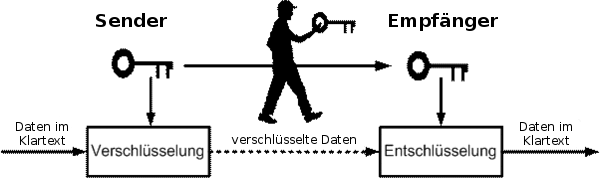
\includegraphics[width=15cm]{images/symmetrischeVerschluesselung.png}
\caption{Symmetrische Verschlüsselung}
\label{fig:symVersch}
\end{center}
\end{figure}
In Abbilding \ref{fig:symVersch} wird ein Klartext mit einem Schlüssel verschlüsselt. Der Schlüssel muss vom Sender an den Empfänger übergeben werden. 
%
%******************************************
%  Asymmetrische Verschlüsselung
%******************************************
\subsection{Asymmetrische Verschlüsselung}
Vor 1970, als es die asymmetrische Verschlüsselung noch nicht gab, wurden Schlüssel für eine symmetrische Verschlüsselung unter grossem Schutz transportiert.
%
%Es waren vor allem die Botschaften, die einen solchen Transport mehrfach absicherten, indem sie dem Überbringer den Koffer mit Handschellen am Handgelenk festmachten und ihn von diversen Bodyguards beschützt in einer kugelsicheren Limousine zum Zielort fuhren.\\
Dieses Verfahren war sehr umständlich. Es kostete viel und dauerte zu lang. Wie aber sollte man einen Schlüssel sicher von einem Ort zum andern transportieren und dabei sicher sein, dass niemand einen Blick auf den Schlüssel werfen konnte?\\
%
Anfang 1976 stellten Whitfield Diffe und Martin Hellman ein Konzept vor, das die Grundidee von einer asymmetrischen Verschlüsselung darlegte. Sie kannten das Verfahren jedoch nicht exakt. Sie stellten das \textbf{Diffle-Hellman-Problem} vor. \cite{rsa_and_public_key}\\ % Stellten das Prinzip vor
Schon viel früher entwickelten James Ellis, Clifford Cockes und Malcom Willamson, alle vom Britischen Geheimdienst, ein asymmetrisches Verschlüsselungsverfahren. Sie durften aber ihre Ergebnisse weder veröffentlichen noch ein Patent anmelden. 
Der Erfolg gelang Ronald L. \textbf{R}ivest, Adi \textbf{S}hamir und Leonard M. \textbf{A}dleman im Jahre 1977. Sie entwickelten den RSA-Algorithmus.\\[2ex]
%
Bei einem asymmetrischen Verfahren kann der Sender dem Empfänger eine verschlüsselte Nachricht senden, die nur der Empfänger entschlüsseln kann.\\
%
Das funktioniert dank einem öffentlichen Schlüssel, dem \textbf{Public-Key}, und einem privaten Schlüssel, dem \textbf{Private-Key}. Beide zusammen bilden das Schlüsselpaar.\\
Für dieses Verfahren hat sich der Name \textbf{Public Key-Kryptographie} durchgesetzt.
%
% Bei der Formel für die verschlüsselung ist f_e und m verantwortlich für c das heisst es sind beide wichtig!!
%
Um jemandem eine verschlüsselte Nachricht zu senden, benötigt man den öffentlichen Schlüssel des Empfängers. Mit diesem öffentlichen Schlüssel und der Verschlüsselungsfunktion wird der Klartext in ein Chiffrat übersetzt. Nur der Besitzer des privaten Schlüssels ist in der Lage, aus dem Chiffrat den Klartext zu erzeugen.\\
Die Verschlüsselung in einer Formel ausgedrückt:
%Aus dieser Idee kann man eine Funktion erstellen, die das Verschlüssen schematisch darstellt.\\
\begin{equation*}
  c = f_e (m)
  \label{eqn:asy_versch}
\end{equation*}
Der Verschlüsselungsalgorithmus \textit{f} verschlüsselt den Klartext \textit{m} in den verschlüsselten Text \textit{c} mit Hilfe des Verschlüsselungs-Exponenten \textit{e} (eng.: \textit{encription exponent}).\\
% c = f(e,m)
%\paragraph{Entschlüsseln}
%Der Empfänger empfängt den verschlüsselten Text und entschlüsselt ihn mit Hilfe seines privaten Schlüssel und erhält den Klartext.
%Auch hier läst sich dieses Vorgehen in einer Funktion beschreiben.\\
%Mit der Entschlüsselungsfunktion f und dem privaten Schlüssel d wird aus dem verschlüsseltem Text c den Klartext m' gewonnen.
Die Entschlüsselung in einer Formel ausgedrückt:
\begin{equation*}
  m' = f_d (c) 
  \label{eqn:asy_entsch}
\end{equation*}
Mit der Entschlüsselungsfunktion \textit{f} und dem Entschlüsselungs-Exponenten \textit{d} (eng.: \textit{decription exponent}) wird aus dem verschlüsseltem Text \textit{c} den Klartext \textit{m'} gewonnen.
%
%Das Wichtigste bei der asymmetrischen Verschlüsselung ist, dass beim Entschlüsseln wieder der \textbf{gleiche} Text reproduziert wird, auch wenn zum Ver- und Entschlüsseln zwei unterschiedliche Schlüssel verwendet wurden.\\
%Der ganze Vorgang in einer Gleichung ausgedrückt (c parametrisiert):
%\begin{equation*}
%  m' = f_d (c) = f_d (f_e (m) ) = m \\
%  \label{eqn:asy_togh}
%\end{equation*}
%gekürzt\\
%\begin{equation*}
%  m = f_d ( f_e (m) )
%  \label{eqn:asy_togh_shortForm}
%\end{equation*}
%
\begin{figure}[ht]
\begin{center}
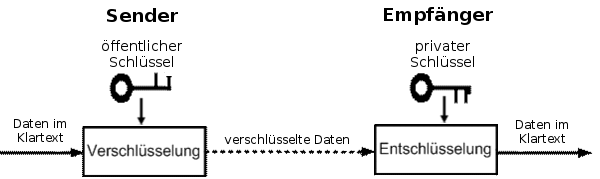
\includegraphics[width=15cm]{images/asymmetrischeVerschluesselung.png}
\caption{Asymmetrische Verschlüsselung}
\end{center}
\end{figure}
%
%\paragraph{Beispiel \footnotemark}
%Herr Müller möchte gern Herrn Spinnler seine sensiblen Daten übergeben. Dafür benötigt er den öffentlichen Schlüssel von Herr Spinnler.\\
%Jetzt verschlüsselt Herr Müller mit dem öffentlichen Schlüssel seine Daten und sendet das Paket an Herrn Spinnler. Dieser wiederum entschlüsselt das Paket mit seinem geheimen, gut aufbewarten, privaten Schlüssel. Jetzt ist er im Stande die Nachricht von Herrn Müller zu lesen.

%\footnotetext{Dieses Beispiel zeigt einen schematischen Ablauf. Es geht nicht auf das Verschlüsselungsverfahren ein.}
% Erwähnen dass man bei der Asymetrischen Verschlüsselung Einwegfunktionen benötigt

%Im wirklichkeit sieht das Verfahren so aus. Eine Person A erstellt zwei Schlüssel. Einen privaten Schlüssel, der nur sie kennt und einen öffentlichen, d%en sie Person B gibt. Jetzt möchte B an A einen Text senden. Hierfür nimmt es den öffentichen Schlüssel von A und verschlüsselt den Text.
%Diesen Verschlüsselten Text sendet Person B an A. 
%A nimmt jetzt den verschlüsselten Text entgegen und entschlüsselt ihn mit Hilfe des privaten Schlüssel.
%Da A nur den privaten Schlüssel hat, mit der sich den verschlüsselten Text entschlüsseln lässt, kann nur A den Text lesen.
%Der Empfänger erstellt zwei Schlüssel. Einen öffentlichen den er verteilen kann und einen geheimen privaten Schlüssel denn er keinem zeigt. 
